\documentclass[12pt]{article}

\usepackage{graphicx}
\usepackage[margin=1.25in]{geometry}
\usepackage{multirow}

\usepackage{amsmath}
\usepackage{bm}
\newcommand{\m}[1]{\mathbf{\bm{#1}}}

\begin{document}

\section*{Project 2 -- AMS 276}
\subsection*{Mickey Warner}
\bigskip
\bigskip

\noindent We ran each simulation to completion (until $n > N_{max}$), but where the trial would have ended is marked with a vertical line. The color of the vertical line indicates the reason for the stopping: red is for excessive toxicity, green is for futility, and blue is for both.
\bigskip

\noindent Scenario 1 has a true probability of toxicity being larger (0.4) than efficacy (0.2). In this case, we expect to stop the trial early. Of the five simulations presented, two stopped early due to toxicity, two for non-efficacy, and one for both. It can be seen that variability is high, especially early on in the study. With many simulations, only a very few ran to completion.
\bigskip

\noindent Scenario 2 is the opposite of the first. Here, an efficacy event has probability 0.4 while toxicity has 0.2. As in the first scenario, there is a lot of variability early in the study. This is concerning since we may stop the study early when we really shouldn't. In one of the simluations, we stopped after the second cohort was tested, but should the trial continue, the probability of toxicity drops dramatically.
\bigskip

\noindent The variability can even be seen to persist through near the end of the study as well. One simulation ended early because efficacy was too low (below 0.02), but had the trial continued we would see the probability of an efficacy event rise toward 0.4.
\bigskip

\noindent This could issue be dealt with by specifying a minimum number of cohorts to test. Since the variability is reduced as more patients are tested, we would have a lower chance of incorrectly stopping a study early.
\bigskip

\noindent Furthermore, some things were said in class about two lines and their removal in the

\newpage

\begin{figure}[ht]
\centering
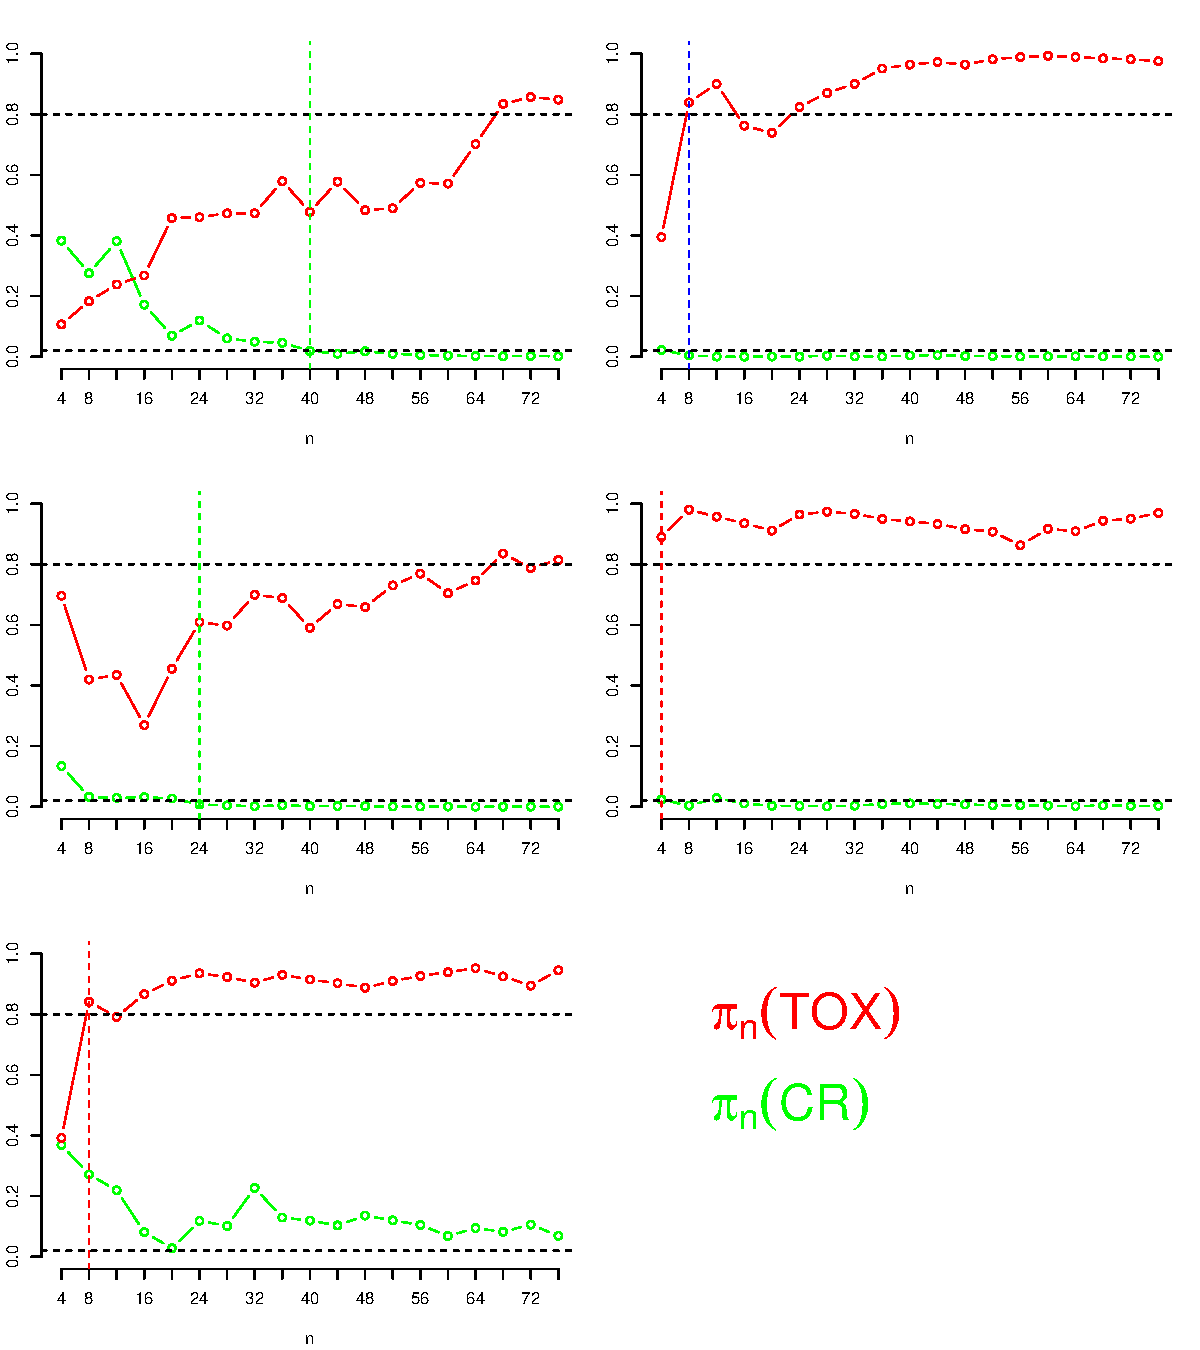
\includegraphics[scale=0.75]{figs/scen1.pdf}
\caption{Five simulations from scenario 1.}
\end{figure}

\newpage

\begin{figure}[ht]
\centering
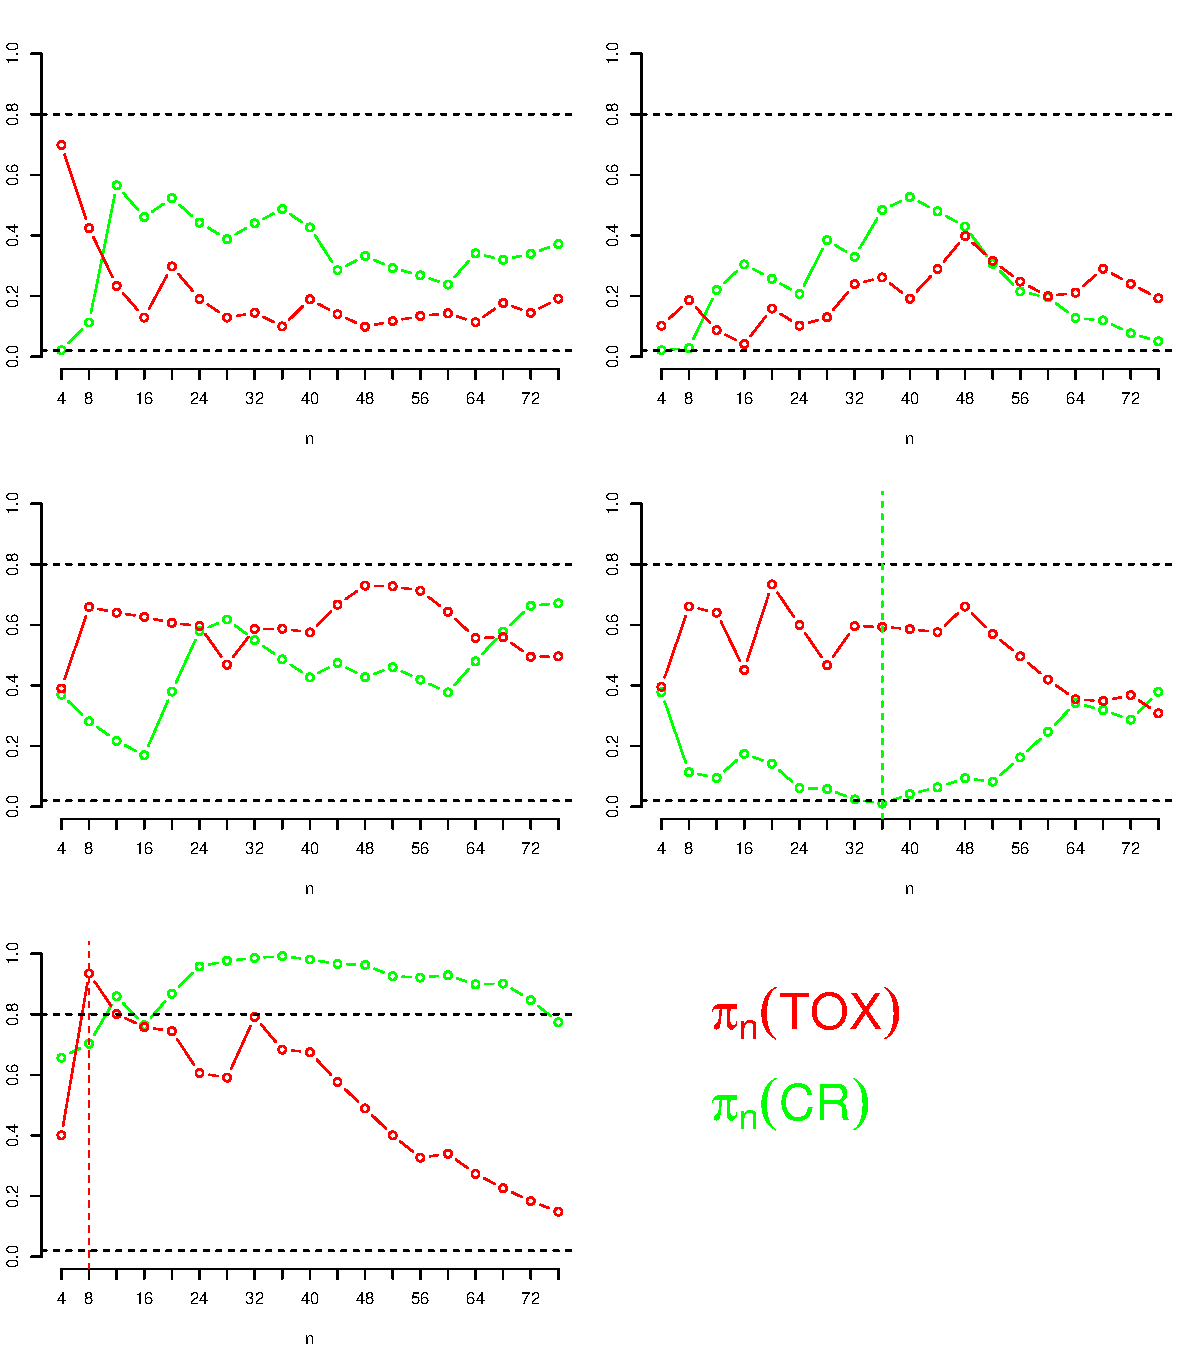
\includegraphics[scale=0.75]{figs/scen2.pdf}
\caption{Five simulations from scenario 2.}
\end{figure}

\end{document}
